\chapter{\uppercase {OpenFlow Extensions}}
\label{sec:extensions}

\blfootnote{*This  work is based upon paper titled "\aetherflow: Principled Wireless Support in SDN" published in CoolSDN '15 ~\cite{aetherflow} and the paper titled "\crossflow: A Cross-layer Architecture for SDR using SDN principles" published in IEEE NFV-SDN '15.~\cite{crossflow}}

In our previous work, we derived a generalized SDN abstractions model, called
TinyNBI \cite{Casey:14}, from the OpenFlow specifications \cite{openflow}.
In TinyNBI, the OpenFlow data plane is composed of
several elements. The data plane elements and their structural relationships are
depicted as UML diagram in Figure~\ref{fig:data_model}. TinyNBI model provides a 
clean low-level interpretation of the core OpenFlow abstractions and supports 
development of higher layer abstractions through refinement or extension.
The model is primarily based on the notion of resources shared across a
data plane. 

% A data plane receives packets from a set of different ports, and
% forwards those to a pipeline, defined largely by table lookups and their
% associated actions, for processing and forwarding.

\begin{figure}[t]
  \centering
  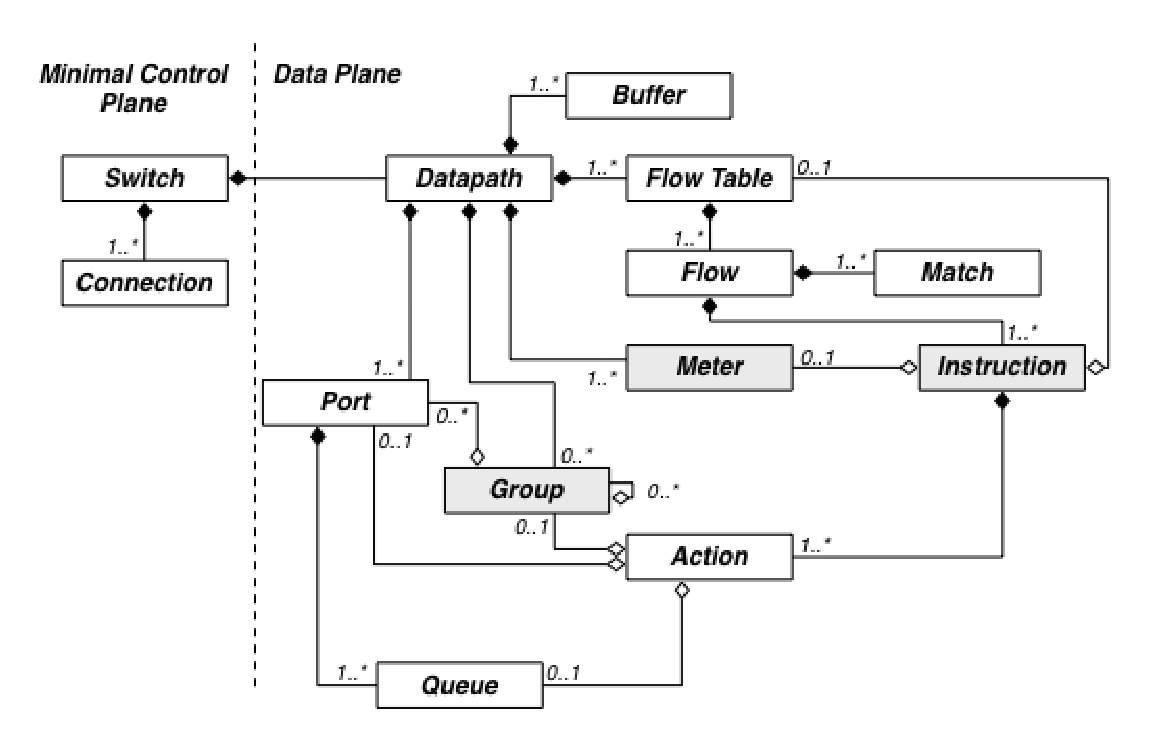
\includegraphics[scale=0.64]{figures/data_model.pdf}
  \caption[UML diagram of OpenFlow data model]{A UML diagram of OpenFlow data model. Each box represents a data
  plane element and the lines show the dependencies relationship among the
  elements.}{[Reprinted\space from\space \textsuperscript{\cite{flowgrammable}}]}
  \label{fig:data_model}
\end{figure}

\begin{figure}[t]
  \centering
  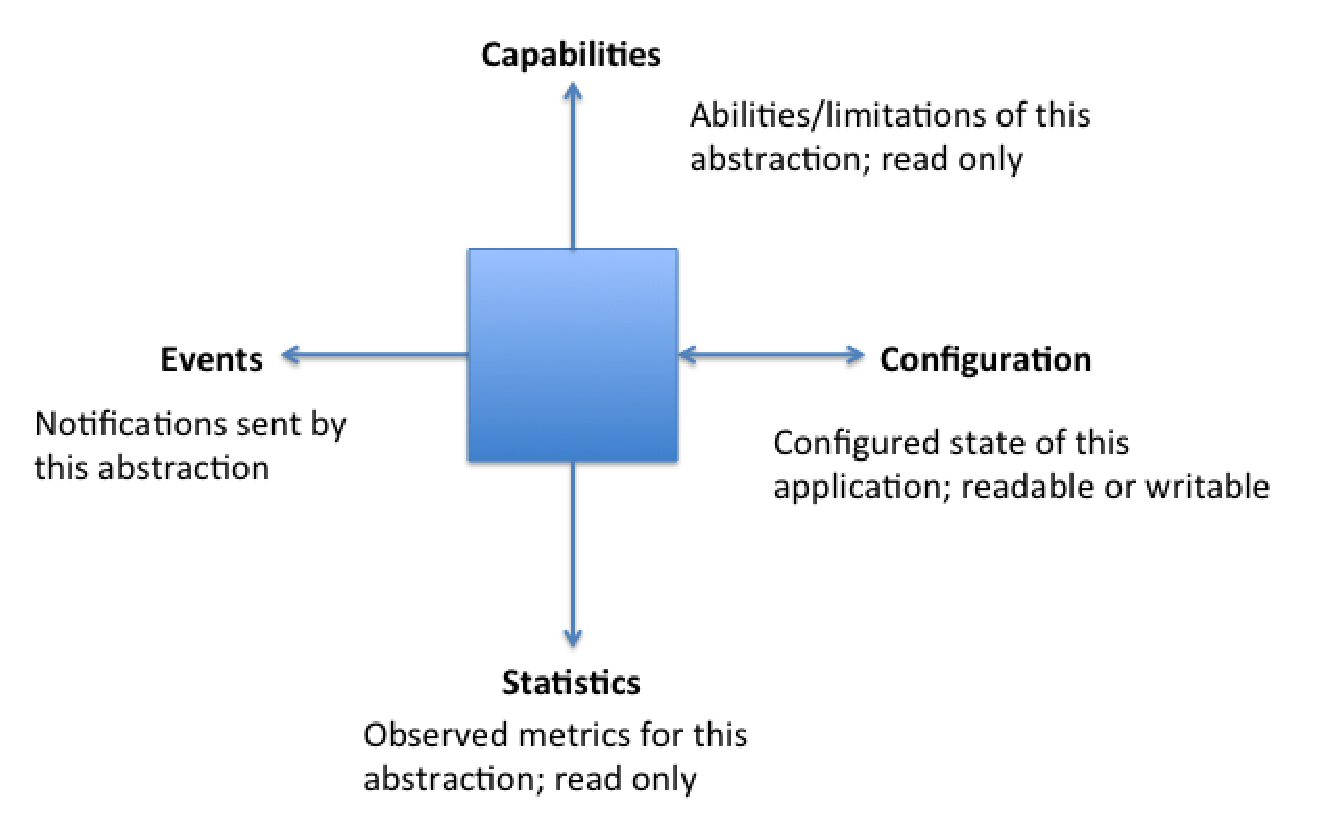
\includegraphics[scale=0.64]{figures/abstraction.pdf}
  \caption{OpenFlow interfaces abstraction.}
  \label{fig:abstraction}
\end{figure}

In the TinyNBI model, each component exposes four types of interfaces:
capabilities, configuration, statistics and events.  These interfaces and their
information flow directions are conceptually depicted in
Figure~\ref{fig:abstraction}.

\textbf{Capabilities.} Not every switch provides the same level of
support for e.g., matching on protocol fields. Each component in the
model must provide a facility that allows a controller to discover the
set of operations supported by the device.

\textbf{Configuration.} Each OpenFlow data model element has some
configurable parameters that can be modified during switch operation.
The configuration interfaces are used to modify state and behavior of the data
model element. 

\textbf{Statistics.}  OpenFlow switches gather statistical information
via counters such as the numbers of bytes received and transferred over a
port. Statistics interfaces provide the controller with access to the current
state and values of these counters. 

\textbf{Events.} The events interface reports to the controller certain
types of events that occur during switch operation. 


%\footnotetext{Courtesy: flowgrammable.org}

\section{\aetherflow Data Plane Abstractions}


In order to support wireless networks, we refine the notion of ports from
the TinyNBI SDN model. The SDN model already has a distinction between
physical and logical ports. A \emph{physical port} corresponds to an actual
interface (e.g., Ethernet card), whereas a \emph{logical port} is typically
defined by software. Logical ports are often used for protocol
tunneling and link aggregation.

To support wireless SDN controllers we introduce new types of both physical
and logical ports. \aetherflow introduces wireless physical port
corresponding to an IEEE~802.11 (commonly known as WiFi) radio interface.
This allows controllers to query and configure the physical device over
which packets are sent and received.

Because a single 802.11 radio interface can support multiple simultaneous
wireless access points (APs), \aetherflow also introduces wireless
logical port. Each wireless logical port is associated with its underlying
physical port.

For packet processing, whenever a packet from a wireless AP is
processed, its metadata records its \emph{input port} as the logical port
for the AP and its \emph{input physical port} as the physical port the AP is
created on. The frames received on
the wireless interface are adapted into regular Ethernet frames for pipeline
processing, meaning that we
do not have to define any new protocol matching features for 802.11 MAC frame
fields. This also allows an existing SDN implementation to compose
wireless logical ports into link aggregation ports or various forms of
tunnels.
% 
% Note that we could readily extend the matching capabilities for table
% abstractions to support frames received directly from a physical port.
% We reserve this for future work.

The new data plane elements (wireless ports) defined in \aetherflow expose to
the controller a set of control interfaces, categorized in the same way as the
TinyNBI model, which are described as below.

\textbf{Capabilities.}
\aetherflow allows the controller to query and obtain the capabilities of the
radio interfaces of an AP. The supported capabilities information for wireless
physical port includes 
% contains:
% \begin{itemize}
%   \item Wireless physical port: 
    (i) IEEE~802.11 version; 
    (ii) channels; 
    (iii) transmission power; 
    (iv) encryption and key management methods; 
    (v) maximum number of APs supported.
%\end{itemize}
\aetherflow does not define capabilities interface for wireless logical port.

\textbf{Configuration.}
An OpenFlow controller can use \aetherflow messages to create or remove AP and
dynamically 
(re)configure the following properties of an AP:
\begin{itemize}
  \item Wireless physical port: 
     (i) IEEE~802.11 version; 
    (ii) channel; 
    (iii) transmission power. 

  \item Wireless logical port: 
    (i) SSID; 
    (ii) BSSID; 
    (iii) encryption and key management method.
\end{itemize}

In addition, \aetherflow allows the controller to change the state of mobile
stations associated with it, e.g., drop a station. Any new configuration to an
AP is immediately applied. The configuration interfaces provide
a high degree of programmability to applications that require these parameters 
to be adjusted during network operation.

\textbf{Events.}
  An SDN controller can receive MAC layer events related to a mobile station. 
  \aetherflow currently supports the following types of
  events for wireless logical port:
  % \begin{itemize}
  %    \item Wireless logical port: 
      (i) probe; 
      (ii) authentication; 
      (iii) deauthentication; 
      (iv) association; 
      (v) reassociation; 
      (vi) disassociation; 
      (vii) authorization.
  %\end{itemize}
\aetherflow does not define any event interface for wireless physical port.
 % No event interface is defined for wireless physical port.

  The events occur when AP receives the corresponding 802.11 management frames.
  With these events reported, the controller can keep track of the 802.11 state
  of all the mobile stations communicating with the APs under control. 

\textbf{Statistics.}
  An SDN controller can query the statistics of each physical wireless
  port and its associated logical ports. For a wireless logical port the following types
  of statistics are supported: 
  % \begin{itemize}
  %    \item Wireless logical port: 
      (i) number of packets sent and received; 
      (ii) number of bytes sent and received; 
      (iii) number of retries;
      (iv) number of retry failures; 
      (v) current signal strength of a station; 
      (vi) average signal strength of a station; 
      (vii) connection duration of a station.
 %   \item Wireless physical port:
For wireless physical port the set of supported statistics is identical to that supported by the OpenFlow protocol. 
% 
% 
% \aetherflow  from the OpenFlow statistics interface model.
 % \end{itemize}


\section{\aetherflow Messages}
To implement \aetherflow in the framework of OpenFlow, we use experimenter
messages provided in OpenFlow protocol to carry \aetherflow messages. In the current
version, nine messages are defined in \aetherflow:
\begin{itemize}
\item Event report message -- notify controller of events.
\item Logical port statistics request/reply -- request and reply of current 
      statistics from a logical port.
\item Physical port configuration request -- modify the configuration of a
      physical port.
\item Logical port configuration request -- modify the configuration of a
      logical port.
\item Physical port capabilities request/reply -- request and reply of 
      capabilities of a physical port.
\item Drop station -- force a mobile station to disassociate.
\item Error message -- customize error reporting for wireless.
\end{itemize}
% The detailed definitions of the messages are omitted due to space limit.
%  For the counters, the switch keeps one counter for each station and each type
%  of statistics. The counter may be turned on or off by the controller. If
%  turned on, the counter gets updated when a corresponding event happens. Signal
%  strength of the client is measured and updated when a frame is received from
%  the corresponding station. Connection state refers to the state of the mobile
%  station in the 802.11 MLME state machine (unauthenticated/unassociated,
%  authenticated/unassociated, authenticated/associated/pending RSN
%  authentication and authenticated/associated).

\section{\crossflow Data Plane Abstractions}

%\begin{figure}[t]
%  \centering
%  \includegraphics[width=0.48\textwidth]{figures/Interfaces.pdf
%  \caption{Interface model for wireless radio port abstraction with two processing blocks: Sink and Modulators}
%  \label{fig:interface}
%\end{figure}

\begin{figure}[t]
  \centering
  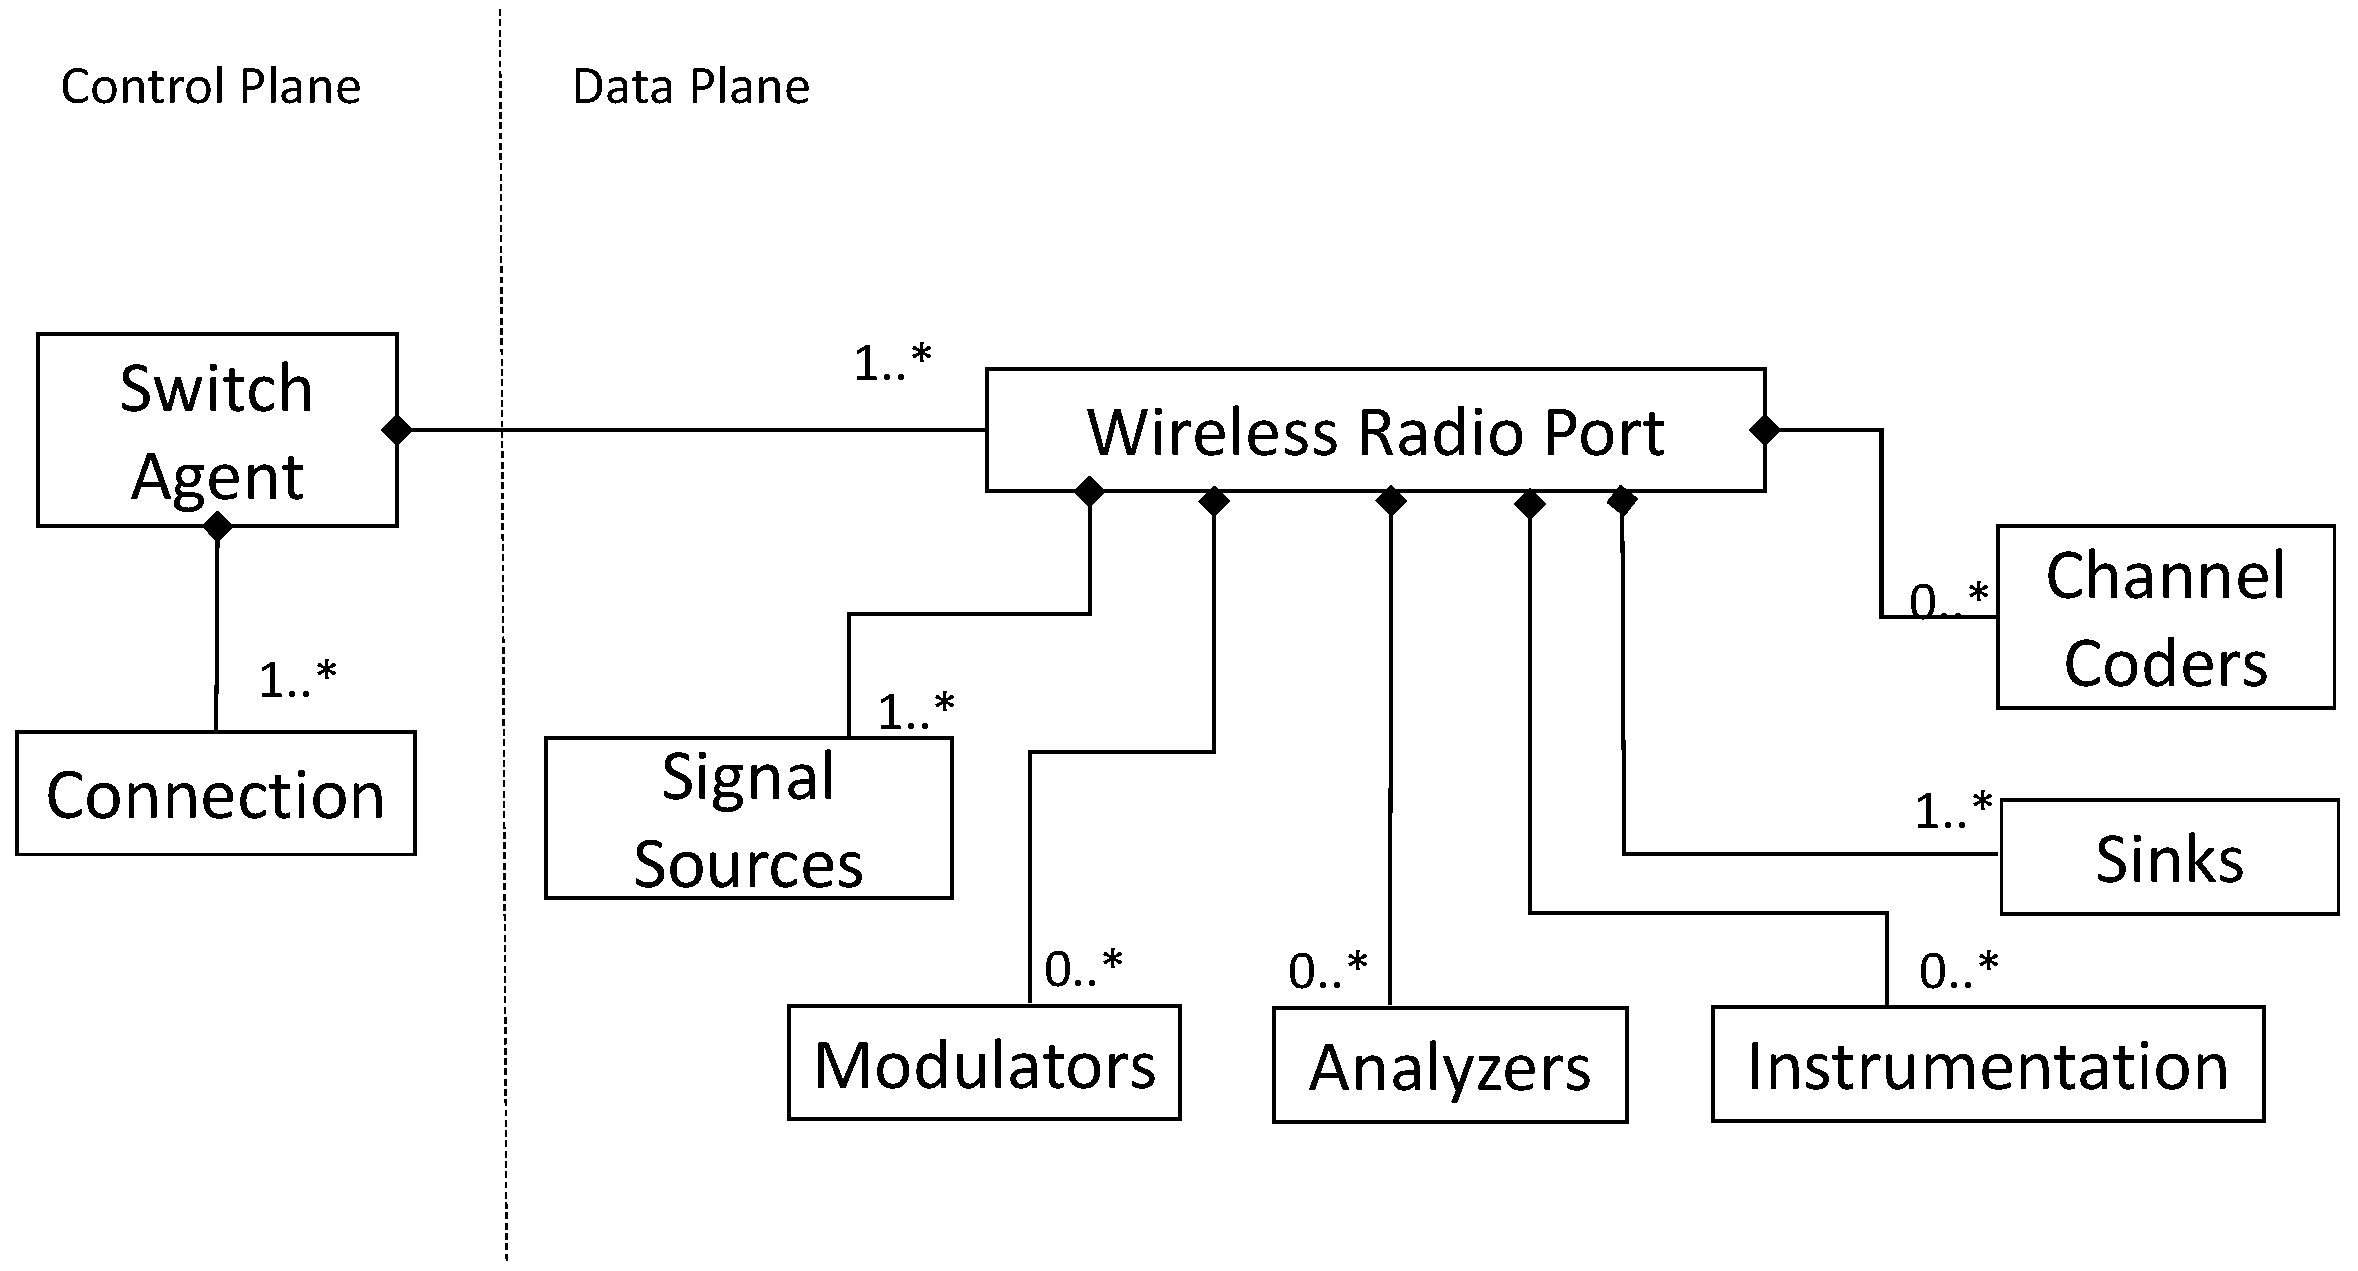
\includegraphics[width=0.8\textwidth]{figures/UML.pdf}
  \caption{UML diagram of \crossflow model.}
  \label{fig:uml}
\end{figure}

%\begin{figure*}
%  \centering
%  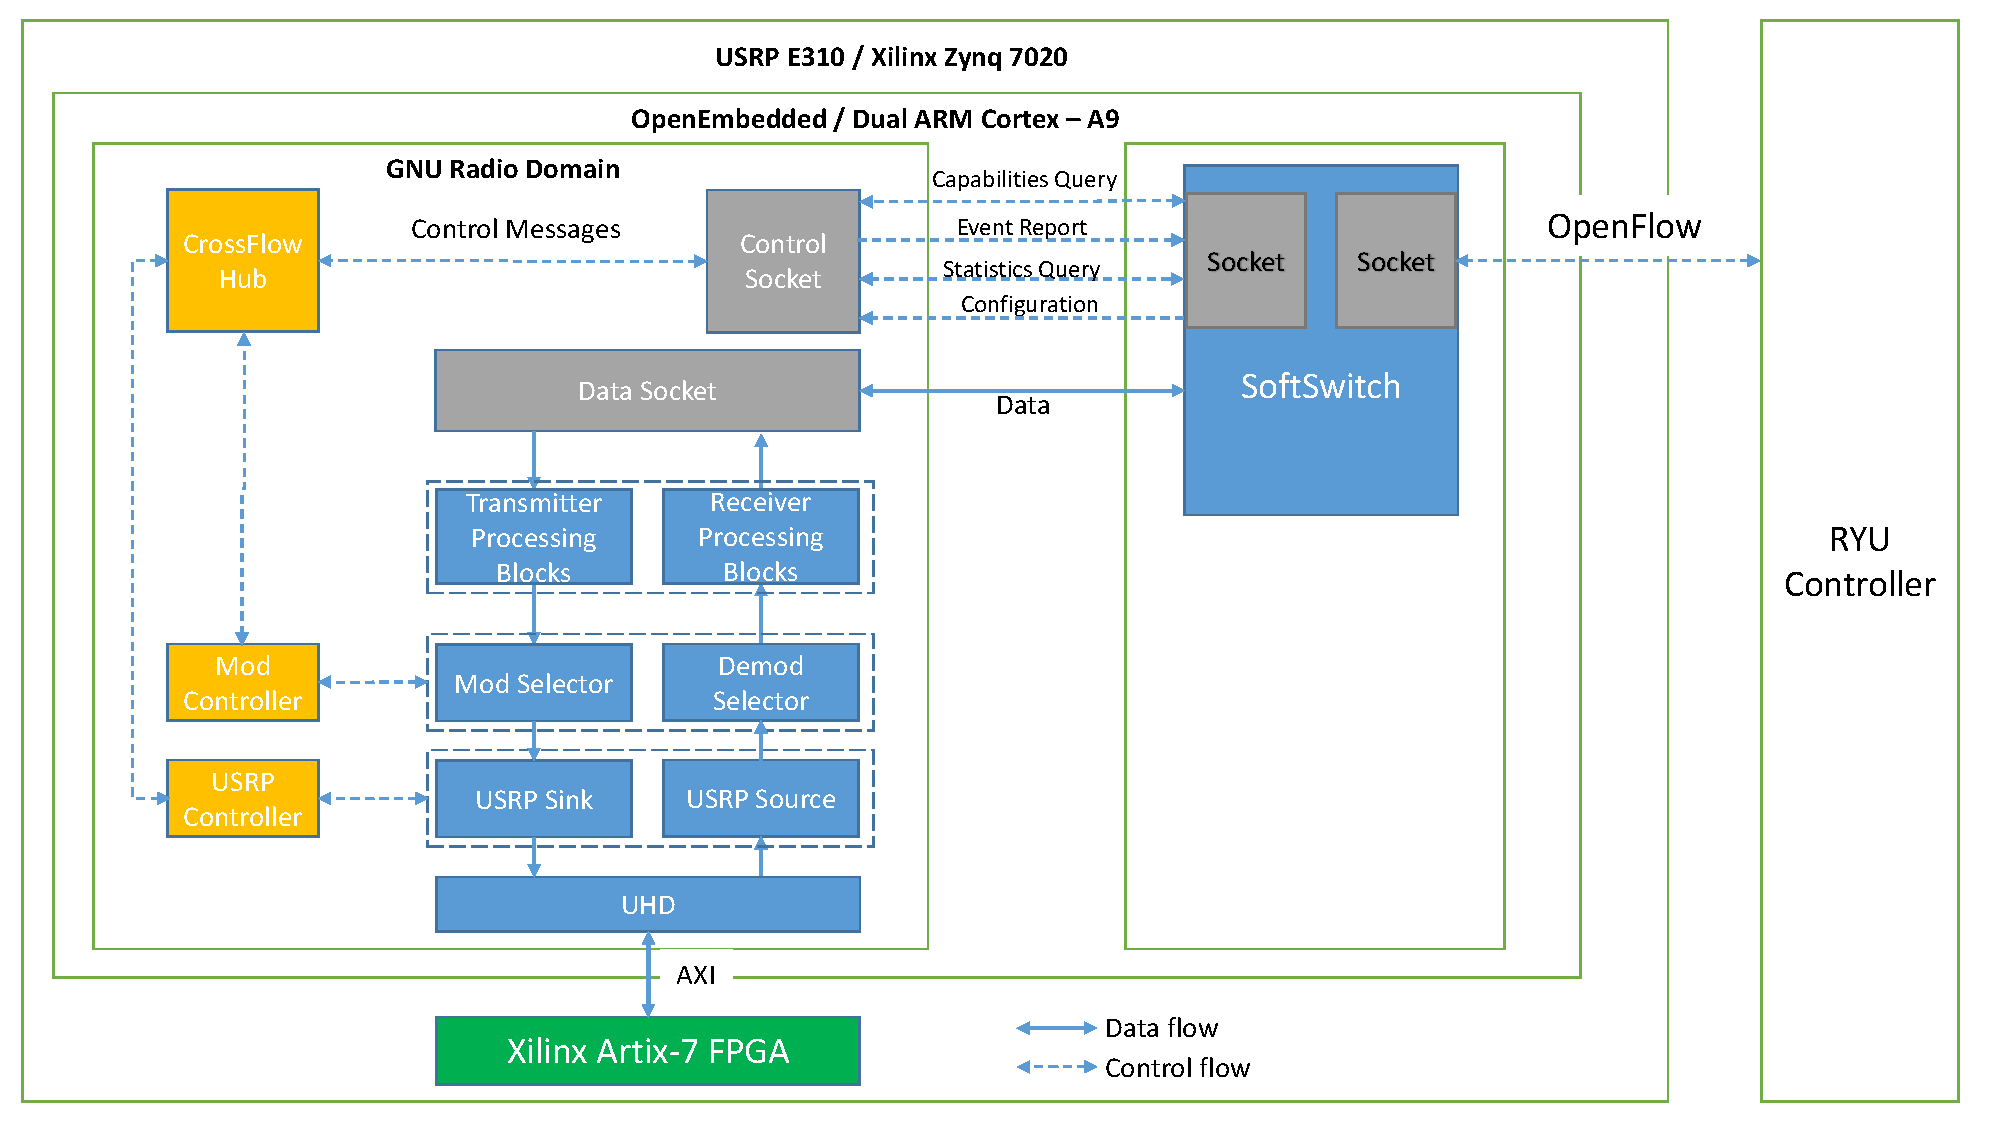
\includegraphics[width=0.8\textwidth]{figures/new.pdf}
%  \caption{Implementation of \crossflow}
%  \label{fig:message_block}
%\end{figure*}

We extend the data model proposed in \cite{Casey:14} to create an abstraction model for the \crossflow framework, which is displayed in Figure~\ref{fig:uml}. We build upon the \emph{radio physical port} concept proposed in \cite{aetherflow} to create a new layer of abstractions, which we refer to as the \emph{wireless radio port} in this paper. This layer of abstractions exhibits a composition or \emph{has-a} relationship with the \emph{wireless radio port} abstraction (i.e., ``the wireless radio port \emph{has a} sink, modulator, or channel coder). This means that the blocks of this layer are the objects or members that comprise the \emph{wireless radio port}. These blocks are derived from the most commonly used processing blocks in GNU Radio~\cite{gnuradio}. This abstract wireless radio port model serves the following design vision:

\begin{itemize}
\item It allows visibility into the signal processing blocks from an application point of view, without going into implementation details.
\item It allows for the development of an event driven framework for radio operation.
\item It allows composition of blocks to implement new functionality, as this decision is handled by the higher \emph{radio physical port} abstraction. The application simply specifies the blocks to be connected for a specific wireless port instance and the internal framework handles the implementation.
\end{itemize}

In our current design, we focus on the first point of changing and quering the parameters of blocks at runtime. We assume that the number of blocks is fixed and the blocks can be connected in a consistent manner. In order to change parameters, the application needs to send \emph{\big \langle command,value\big \rangle} tuple in a message. For query and receive event responses, it registers for events for each block and during an event, appropriate callbacks are invoked. This ability to register for events is important so that a centralized controller can receive events asyncronously and implement a reactive model for its operations.
    
One of the main requirements of the \crossflow model is that each abstraction should implement four types of interfaces as proposed in \cite{Casey:14}, namely: capabilities, configuration, statistics and events. The interface model for \crossflow provides the interfaces for a wireless radio port abstraction with only two processing blocks, \emph{Sink} and \emph{Modulators}. The Sink abstraction allows the controller to manage the signal sinks which can be a USRP device, file or a socket, while the Modulators abstraction allows management of modulation schemes (e.g., BPSK, QPSK, and 8PSK).

The interfaces for \emph{Sink} and \emph{Modulators} are categorized as follows:

%\textbf{Capabilities.}
\textbf{Sink.}
\begin{itemize}
\item \textbf{Capabilities}: The interface allows the controller to query the capabilities of sinks such as:
    (i)  Type of sink (USRP, socket, etc.);
    (ii) Channels supported; 
    (iii) Center Frequency; and
    (iv) IP address. 
\item \textbf{Configuration}: The interface allows the controller to configure properties of signal sinks such as:
    (i) Gain;
    (ii) Frequency, and
    (iii) Sample rate.
\item \textbf{Statistics}: The interface allows the controller to gather statistics for sinks such as:
    (i) Received Signal Strength Indicator (RSSI) and 
    (ii) Temperature on-board.
\item \textbf{Events}: The interface allows the controller to take decisions based upon events in a sink such as:
    (i) Low or high RSSI and
    (ii) Low or high on-board temperature.
\end{itemize}

\textbf{Modulators.}
\begin{itemize}
\item \textbf{Capabilities}: The interface allows the controller to query the properties of the modulator block such as:
    (i) Modulations supported;
    (ii) Current samples/symbol; and
    (iii) Gray code.
\item \textbf{Configuration}: The interface allows the controller to configure properties of the modulator block such as:
    (i) Choice of modulation scheme (e.g. BPSK, QPSK and 8PSK);
    (ii) Samples/symbol; and
    (iii) Use of a Gray code.
\item \textbf{Statistics}: The interface allows the controller to gather statistics for the modulator block such as:
    (i) Signal to Noise Ratio (SNR) and 
    (ii) Bit Error Rate (BER).
\item \textbf{Events}: The interface allows the controller to take decisions based upon events in the modulator block such as:
    (i) Low or high SNR and
    (ii) Low or high BER.
\end{itemize}

\section{\crossflow Message Extensions}
\label{sec:messages}
  		  
\crossflow uses SDN design principles to control a network of configurable SDRs. As such, to enable control plane interactions between the SDN controller and the SDR, we had two options: either we could have implemented our own control protocol to enable their interactions or extend the existing OpenFlow \cite{openflow} framework. This is because OpenFlow does not natively support wireless features. In order to enable a cleaner implementation, we extend OpenFlow by using experimenter messages within the OpenFlow protocol, similar to \aetherflow. This provides two advantages:
\begin{itemize}
\item We do not need to implement a new protocol for control and data plane interactions.
\item As we are using experimenter messages to carry \crossflow messages, the controller does not need to perform special handling for these messages. This enables the controller to remain independent of the underlying devices and hence it can handle both wired and wireless devices. 
\end{itemize} 
We currently define configuration request messages for the Sink and Modulators abstractions.
